\SetSlideHeaderLevel{section}

% =============================================
\section{Pengantar: Perjalanan Pembelajaran Progresif}
% =============================================

\begin{frame}[t, fragile]
    \frametitle{Week 09: Game Loop \& Singleton Pattern}
    \footnotesize
    \begin{spacing}{0.85}
    \begin{columns}[T]
        \begin{column}{0.50\textwidth}
            \textbf{Tujuan Pembelajaran:}
            \begin{itemize}
                \item Memahami \textbf{Game Loop Pattern}
                \item Memisahkan update dan rendering
                \item Mengidentifikasi anti-pattern \textbf{Object Drilling}
                \item Mengimplementasikan \textbf{Singleton Pattern}
                \item Menganalisis trade-off arsitektur
            \end{itemize}

            \vspace{0.5cm}

            \textbf{Pendekatan Pembelajaran:}
            \begin{itemize}
                \item Progresif: Setiap branch menyelesaikan masalah sebelumnya
                \item Problem-first: Tunjukkan masalah, baru solusi
                \item Evidence-based: Gunakan metrik konkret (FPS, LOC)
            \end{itemize}
        \end{column}

        \begin{column}{0.50\textwidth}
            \centering
            \textbf{Perjalanan 4 Branch}
            \vspace{0.3cm}

            \resizebox{\textwidth}{!}{
            \begin{tikzpicture}[
                node distance=1.8cm,
                block/.style={rectangle, draw, thick, rounded corners, text width=4cm, align=center, minimum height=1.2cm},
                problem/.style={fill=red!20},
                solution/.style={fill=green!20},
                arrow/.style={->, >=Stealth, thick}
            ]
                \node[block, problem] (b00) {\textbf{09-00} \\ Monolithic \\ (Masalah)};
                \node[block, solution, below of=b00] (b01) {\textbf{09-01} \\ Game Loop \\ (Solusi 1)};
                \node[block, problem, below of=b01] (b02) {\textbf{09-02} \\ Object Drilling \\ (Masalah Baru)};
                \node[block, solution, below of=b02] (b03) {\textbf{09-03} \\ Singleton \\ (Solusi Final)};

                \draw[arrow] (b00) -- (b01);
                \draw[arrow] (b01) -- (b02);
                \draw[arrow] (b02) -- (b03);
            \end{tikzpicture}
            }
        \end{column}
    \end{columns}
    \end{spacing}
\end{frame}

% =============================================
\section{Branch 09-00: Masalah Monolithic}
% =============================================

\begin{frame}[t, fragile]
    \frametitle{Branch 09-00: Desain Monolithic}
    \footnotesize
    \begin{spacing}{0.85}
    \begin{columns}[T]
        \begin{column}{0.45\textwidth}
            \textbf{Apa itu Monolithic?}
            \begin{itemize}
                \item Semua kode dalam satu method \texttt{main()}
                \item 150+ baris dalam satu method
                \item Update logic tercampur dengan rendering
                \item Tidak ada separation of concerns
            \end{itemize}

            \vspace{0.5cm}

            \textbf{Masalah yang Ditimbulkan:}
            \begin{itemize}
                \item \textbf{Frame rate coupling}: Rendering lambat $\to$ logic lambat
                \item \textbf{Untestable}: Tidak bisa test tanpa rendering
                \item \textbf{Poor maintainability}: 150+ baris sulit dipahami
                \item \textbf{No scalability}: Menambah entity = slowdown eksponensial
            \end{itemize}
        \end{column}

        \begin{column}{0.55\textwidth}
            \centering
            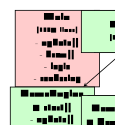
\includegraphics[width=\textwidth]{../../diagrams/uml-comparison.pdf}

            \vspace{0.3cm}

            \begin{alertblock}{Dampak Kritis}
                \textbf{2 FPS} achieved! \\
                Rendering delay 50ms menyebabkan game logic 80\% lebih lambat.
            \end{alertblock}
        \end{column}
    \end{columns}
    \end{spacing}
\end{frame}

\begin{frame}[t, fragile]
    \frametitle{Branch 09-00: Struktur Kode Monolithic}
    \footnotesize
    \begin{spacing}{0.85}
    \begin{columns}[T]
        \begin{column}{0.55\textwidth}
            \begin{minted}[fontsize=\scriptsize]{java}
public class Main {
    public static void main(String[] args) {
        // Initialize
        NPC npc = new NPC();
        Coin coin = new Coin();
        boolean running = true;

        while (running) {
            // Update logic
            npc.move();
            coin.fall();

            // Check collisions
            if (npc.collidesWith(coin)) {
                score += 10;
            }

            // Render (SLOW - menyebabkan masalah!)
            clearScreen();  // 50ms delay!
            drawNPC(npc);
            drawCoin(coin);
            Thread.sleep(50);  // Flickering!
        }
    }
}
            \end{minted}
        \end{column}

        \begin{column}{0.45\textwidth}
            \textbf{Analisis Masalah:}

            \vspace{0.3cm}

            \begin{tabular}{|l|r|}
                \hline
                \textbf{Metrik} & \textbf{Nilai} \\
                \hline
                Lines of Code & 150+ \\
                FPS & 2 \\
                Test Coverage & 0\% \\
                Maintainability & Sangat Rendah \\
                \hline
            \end{tabular}

            \vspace{0.5cm}

            \begin{alertblock}{Masalah Utama}
                \textbf{Tidak bisa unit test!} \\
                Logic tidak bisa ditest tanpa memicu rendering.
            \end{alertblock}
        \end{column}
    \end{columns}
    \end{spacing}
\end{frame}

% =============================================
\section{Branch 09-01: Solusi Game Loop}
% =============================================

\begin{frame}[t, fragile]
    \frametitle{Branch 09-01: Game Loop Pattern}
    \footnotesize
    \begin{spacing}{0.85}
    \begin{columns}[T]
        \begin{column}{0.45\textwidth}
            \textbf{Solusi: Separation of Concerns}

            Pisahkan kode monolithic menjadi class-class khusus:
            \begin{itemize}
                \item \texttt{GameEngine}: Kontrol game loop
                \item \texttt{GameLogic}: Update game state
                \item \texttt{GridRenderer}: Handle rendering saja
            \end{itemize}

            \vspace{0.5cm}

            \textbf{Konsep Kunci:}
            \begin{itemize}
                \item \texttt{update()} - Logic only
                \item \texttt{draw()} - Rendering only
                \item Delta time ($\Delta t$)
                \item Frame rate independence
            \end{itemize}

            \vspace{0.5cm}

            \textbf{Benefits:}
            \begin{itemize}
                \item Testable (no display needed)
                \item 60 FPS performance
                \item Clean separation
                \item Predictable behavior
            \end{itemize}
        \end{column}

        \begin{column}{0.55\textwidth}
            \centering
            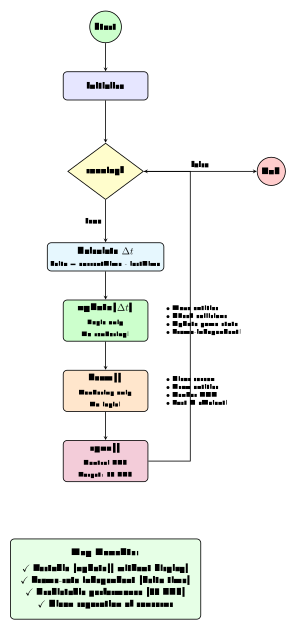
\includegraphics[width=\textwidth]{../../diagrams/game-loop-pattern.pdf}
        \end{column}
    \end{columns}
    \end{spacing}
\end{frame}

\begin{frame}[t, fragile]
    \frametitle{Branch 09-01: Implementasi Game Loop}
    \footnotesize
    \begin{spacing}{0.85}
    \begin{columns}[T]
        \begin{column}{0.55\textwidth}
            \begin{minted}[fontsize=\scriptsize]{java}
public class GameEngine {
    private GameLogic logic;
    private boolean running = true;
    private long lastTime;

    public void start() {
        lastTime = System.currentTimeMillis();

        while (running) {
            long currentTime = System.currentTimeMillis();
            float delta = (currentTime - lastTime) / 1000.0f;
            lastTime = currentTime;

            update(delta);  // Logic only!
            draw();         // Render only!
            sync();         // Control FPS (60 target)
        }
    }

    private void update(float delta) {
        logic.update(delta);
    }

    private void draw() {
        GridRenderer.clearScreen();
        logic.draw();
    }
}
            \end{minted}
        \end{column}

        \begin{column}{0.45\textwidth}
            \textbf{Main.java sekarang SANGAT sederhana:}

            \begin{minted}[fontsize=\scriptsize]{java}
public class Main {
    public static void main(String[] args) {
        GameEngine engine = new GameEngine();
        engine.start();
    }
}
            \end{minted}

            \vspace{0.5cm}

            \textbf{Hanya 3 baris!} Dari 150+ baris menjadi 3 baris.

            \vspace{0.5cm}

            \begin{exampleblock}{Achievement Unlocked!}
                Clean, testable, professional 60 FPS architecture!
            \end{exampleblock}
        \end{column}
    \end{columns}
    \end{spacing}
\end{frame}

\begin{frame}[t, fragile]
    \frametitle{Branch 09-01: Performance Improvement}
    \footnotesize
    \begin{spacing}{0.85}
    \begin{columns}[T]
        \begin{column}{0.50\textwidth}
            \centering
            \textbf{Komparasi 09-00 vs 09-01}

            \vspace{0.5cm}

            \begin{tabular}{|l|r|r|c|}
                \hline
                \textbf{Metrik} & \textbf{09-00} & \textbf{09-01} & \textbf{Change} \\
                \hline
                Lines in Main & 150+ & 3 & \textcolor{green}{50x} \\
                FPS & 2 & 60 & \textcolor{green}{30x} \\
                Testability & 0\% & 100\% & \textcolor{green}{Perfect} \\
                Flickering & Yes & No & \textcolor{green}{Fixed} \\
                \hline
            \end{tabular}

            \vspace{0.5cm}

            \begin{exampleblock}{Hasil}
                \textbf{30x peningkatan FPS!} \\
                \textbf{50x pengurangan kompleksitas!}
            \end{exampleblock}
        \end{column}

        \begin{column}{0.50\textwidth}
            \centering
            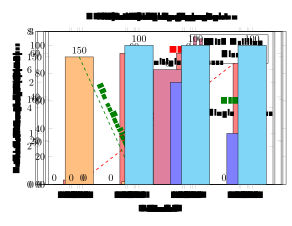
\includegraphics[width=\textwidth]{../../diagrams/performance-comparison.pdf}
        \end{column}
    \end{columns}
    \end{spacing}
\end{frame}

% =============================================
\section{Branch 09-02: Masalah Baru (Object Drilling)}
% =============================================

\begin{frame}[t, fragile]
    \frametitle{Branch 09-02: Ekspansi Game - Requirement Baru}
    \footnotesize
    \begin{spacing}{0.85}
    \begin{columns}[T]
        \begin{column}{0.45\textwidth}
            \textbf{Requirement Baru:}

            Tambahkan HUD (Heads-Up Display) untuk menampilkan:
            \begin{itemize}
                \item Current score
                \item Game time
                \item Player level
            \end{itemize}

            \vspace{0.5cm}

            \textbf{Design Challenge:}

            Multiple class perlu akses \texttt{GameManager}:
            \begin{itemize}
                \item \texttt{GameLogic} $\to$ update score
                \item \texttt{HUD} $\to$ display score
                \item \texttt{NPC} $\to$ check game state
                \item \texttt{Coin} $\to$ add points
            \end{itemize}

            \vspace{0.5cm}

            \textbf{Solusi Naif:}

            Pass \texttt{GameManager} lewat constructor parameters... \textbf{BURUK!}
        \end{column}
        \begin{column}{0.55\textwidth}
            \centering
            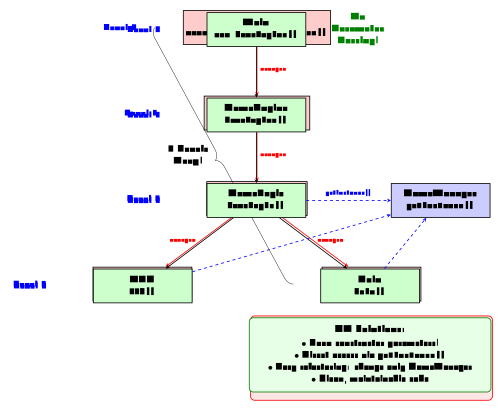
\includegraphics[width=\textwidth]{../../diagrams/object-drilling.pdf}
        \end{column}
    \end{columns}
    \end{spacing}
\end{frame}

\begin{frame}[t, fragile]
    \frametitle{Branch 09-02: Object Drilling Anti-Pattern}
    \footnotesize
    \begin{spacing}{0.85}
    \begin{columns}[T]
        \begin{column}{0.55\textwidth}
            \textbf{Implementasi dengan Object Drilling:}

            \begin{minted}[fontsize=\scriptsize]{java}
// Main.java
GameManager manager = new GameManager();
GameEngine engine = new GameEngine(manager);
engine.start();

// GameEngine.java
public GameEngine(GameManager manager) {
    this.logic = new GameLogic(manager);
    this.hud = new HUD(manager);
}

// GameLogic.java
public GameLogic(GameManager manager) {
    this.npc = new NPC(manager);
    this.coins.add(new Coin(manager));
}

// 4 LEVELS DEEP!
            \end{minted}

            \vspace{0.3cm}

            \textbf{Consequences:}
            \begin{itemize}
                \item 6+ files affected by changes
                \item Team collaboration conflicts
                \item Constructor pollution
                \item Refactoring nightmare
            \end{itemize}
        \end{column}

        \begin{column}{0.45\textwidth}
            \textbf{Bug Kritis!}

            \begin{minted}[fontsize=\scriptsize]{java}
public class HUD {
    // BUG: Creates NEW instance!
    private final GameManager manager
        = new GameManager();

    public HUD(GameManager passedManager) {
        // Ignore parameter!
        System.out.println("Using own instance!");
    }

    public void draw() {
        // Reads from WRONG instance!
        int score = manager.getScore();
        System.out.println("Score: " + score);
    }
}
            \end{minted}

            \begin{alertblock}{Output}
                \texttt{[GameManager:498931366] Score: 10} \\
                \texttt{[HUD] Score: 0}
            \end{alertblock}
        \end{column}
    \end{columns}
    \end{spacing}
\end{frame}

% =============================================
\section{Branch 09-03: Solusi Singleton}
% =============================================

\begin{frame}[t, fragile]
    \frametitle{Branch 09-03: Singleton Pattern}
    \footnotesize
    \begin{spacing}{0.85}
    \begin{columns}[T]
        \begin{column}{0.45\textwidth}
            \textbf{Solusi: Guarantee Single Instance}

            Singleton pattern memastikan class hanya punya SATU instance dan menyediakan global access point.

            \vspace{0.5cm}

            \textbf{Tiga Komponen Kunci:}
            \begin{enumerate}
                \item Private static instance
                \item Private constructor
                \item Public static getInstance()
            \end{enumerate}

            \vspace{0.5cm}

            \textbf{Benefits:}
            \begin{itemize}
                \item Zero constructor parameters
                \item Guaranteed single instance
                \item Global access point
                \item Easy refactoring
            \end{itemize}
        \end{column}

        \begin{column}{0.55\textwidth}
            \centering
            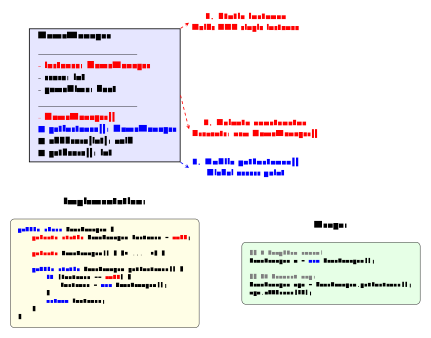
\includegraphics[width=0.9\textwidth]{../../diagrams/singleton-pattern.pdf}
        \end{column}
    \end{columns}
    \end{spacing}
\end{frame}

\begin{frame}[t, fragile]
    \frametitle{Branch 09-03: Implementasi Singleton}
    \footnotesize
    \begin{spacing}{0.85}
    \begin{columns}[T]
        \begin{column}{0.55\textwidth}
            \begin{minted}[fontsize=\scriptsize]{java}
public class GameManager {
    // 1. Static instance (lazy initialization)
    private static GameManager instance = null;

    private int score;
    private float gameTime;
    private int level;

    // 2. Private constructor
    //    (prevents: new GameManager())
    private GameManager() {
        this.score = 0;
        this.gameTime = 0.0f;
        this.level = 1;
        System.out.println("[GameManager]
            Singleton created: " + this.hashCode());
    }

    // 3. Global access point
    public static GameManager getInstance() {
        if (instance == null) {
            instance = new GameManager();
        }
        return instance;
    }

    public void addScore(int points) {
        this.score += points;
    }
}
            \end{minted}
        \end{column}

        \begin{column}{0.45\textwidth}
            \textbf{Usage yang Clean:}

            \begin{minted}[fontsize=\scriptsize]{java}
// Main.java - No parameters!
public class Main {
    public static void main(String[] args) {
        GameEngine engine = new GameEngine();
        engine.start();
    }
}

// HUD.java - Direct access!
public class HUD {
    public HUD() {
        // No parameters needed!
    }

    public void draw() {
        // Guaranteed THE instance
        int score = GameManager
            .getInstance()
            .getScore();
        System.out.println("Score: " + score);
    }
}
            \end{minted}

            \begin{exampleblock}{Result}
                \textbf{Zero object drilling!} \\
                \textbf{Bug fixed!}
            \end{exampleblock}
        \end{column}
    \end{columns}
    \end{spacing}
\end{frame}

% =============================================
\section{Analisis Komparatif}
% =============================================

\begin{frame}[t, fragile]
    \frametitle{Evolusi Arsitektur: 09-00 $\to$ 09-03}
    \footnotesize
    \begin{spacing}{0.85}
    \begin{columns}[T]
        \begin{column}{0.55\textwidth}
            \centering
            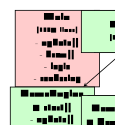
\includegraphics[width=\textwidth]{../../diagrams/uml-comparison.pdf}
        \end{column}

        \begin{column}{0.45\textwidth}
            \textbf{Transformasi Progresif:}

            \vspace{0.3cm}

            \textbf{09-00 $\to$ 09-01:}
            \begin{itemize}
                \item Monolithic $\to$ Separated concerns
                \item 2 FPS $\to$ 60 FPS
                \item Untestable $\to$ 100\% testable
            \end{itemize}

            \vspace{0.3cm}

            \textbf{09-01 $\to$ 09-02:}
            \begin{itemize}
                \item Add new feature (HUD)
                \item Introduces object drilling
                \item Bug: multiple instances
            \end{itemize}

            \vspace{0.3cm}

            \textbf{09-02 $\to$ 09-03:}
            \begin{itemize}
                \item Singleton pattern
                \item Zero parameters
                \item Single instance guaranteed
            \end{itemize}
        \end{column}
    \end{columns}
    \end{spacing}
\end{frame}

\begin{frame}[t, fragile]
    \frametitle{Comprehensive Metrics: All Branches}
    \footnotesize
    \begin{spacing}{0.85}
        \centering
        \begin{tabular}{|l|c|c|c|c|}
            \hline
            \textbf{Metrik} & \textbf{09-00} & \textbf{09-01} & \textbf{09-02} & \textbf{09-03} \\
            \hline
            Lines in Main & 150+ & 3 & 32 & 3 \\
            FPS & 2 & 60 & 60 & 60 \\
            Testability & 0\% & 100\% & 100\% & 100\% \\
            Constructor Params & 0 & 0 & 6 & 0 \\
            GameManager Instances & 0 & 0 & 2 (BUG) & 1 \\
            Object Drilling Depth & N/A & N/A & 4 levels & 0 \\
            \hline
        \end{tabular}

        \vspace{0.5cm}

        \centering
        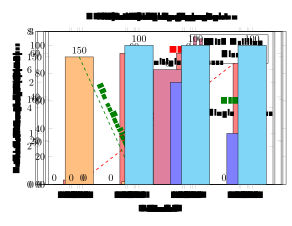
\includegraphics[width=0.7\textwidth]{../../diagrams/performance-comparison.pdf}

        \vspace{0.3cm}

        \begin{exampleblock}{Final Achievement}
            Clean architecture dengan 60 FPS, zero object drilling, dan guaranteed single instance!
        \end{exampleblock}
    \end{spacing}
\end{frame}

% =============================================
\section{Design Patterns Deep Dive}
% =============================================

\begin{frame}[t, fragile]
    \frametitle{Game Loop Pattern: Intent \& Structure}
    \footnotesize
    \begin{spacing}{0.85}
    \begin{columns}[T]
        \begin{column}{0.50\textwidth}
            \textbf{Intent:}

            Decouple the progression of game time from user input and processor speed.

            \vspace{0.5cm}

            \textbf{Structure:}
            \begin{itemize}
                \item \texttt{update(deltaTime)}: Update game state
                \item \texttt{draw()}: Render current state
                \item \texttt{sync()}: Control frame rate
            \end{itemize}

            \vspace{0.5cm}

            \textbf{Participants:}
            \begin{itemize}
                \item \textbf{GameEngine}: Orchestrates the loop
                \item \textbf{GameLogic}: Implements game rules
                \item \textbf{Renderer}: Draws to screen
            \end{itemize}
        \end{column}

        \begin{column}{0.50\textwidth}
            \textbf{Consequences:}

            \vspace{0.3cm}

            \textit{Benefits:}
            \begin{itemize}
                \item Frame-rate independence
                \item Testability tanpa display
                \item Clear separation of concerns
                \item Predictable performance
            \end{itemize}

            \vspace{0.3cm}

            \textit{Liabilities:}
            \begin{itemize}
                \item More classes (increased complexity)
                \item Initial learning curve
                \item Need to manage delta time
            \end{itemize}
        \end{column}
    \end{columns}
    \end{spacing}
\end{frame}

\begin{frame}[t, fragile]
    \frametitle{Singleton Pattern: Intent \& Trade-offs}
    \footnotesize
    \begin{spacing}{0.85}
    \begin{columns}[T]
        \begin{column}{0.50\textwidth}
            \textbf{Intent:}

            Ensure a class has only one instance and provide a global point of access to it.

            \vspace{0.5cm}

            \textbf{When to Use:}
            \begin{itemize}
                \item Shared resource management
                \item Global state needed
                \item Exactly one instance required
            \end{itemize}

            \vspace{0.5cm}

            \textbf{Benefits:}
            \begin{itemize}
                \item Controlled access to sole instance
                \item No global variables
                \item Lazy initialization possible
                \item Easy to refactor
            \end{itemize}
        \end{column}

        \begin{column}{0.50\textwidth}
            \textbf{Liabilities:}
            \begin{itemize}
                \item Global state (testing harder)
                \item Hidden dependencies
                \item Thread safety concerns
                \item Violates Single Responsibility Principle
            \end{itemize}

            \vspace{0.5cm}

            \textbf{Alternatives:}
            \begin{itemize}
                \item \textbf{Dependency Injection}: Pass dependencies explicitly
                \item \textbf{Service Locator}: Registry of services
                \item \textbf{Static Class}: No instantiation needed
            \end{itemize}

            \vspace{0.5cm}

            \begin{alertblock}{Trade-off}
                Singleton menyelesaikan object drilling, tapi introduces global state. Gunakan dengan bijak!
            \end{alertblock}
        \end{column}
    \end{columns}
    \end{spacing}
\end{frame}

% =============================================
\section{Diskusi \& Assessment}
% =============================================

\begin{frame}[t, fragile]
    \frametitle{Discussion Points untuk Kelas}
    \footnotesize
    \begin{spacing}{0.85}
        \textbf{Pertanyaan untuk Mahasiswa:}

        \vspace{0.3cm}

        \begin{enumerate}
            \item Mengapa frame rate coupling adalah masalah kritis dalam game?
            \item Apa trade-off dari Singleton pattern?
            \item Kapan Anda TIDAK akan menggunakan Singleton?
            \item Bagaimana delta time memungkinkan frame-rate independence?
            \item Apa alternatif selain Singleton untuk mengatasi object drilling?
        \end{enumerate}

        \vspace{0.5cm}

        \textbf{Critical Thinking:}

        \vspace{0.3cm}

        \begin{itemize}
            \item Apakah global state selalu buruk?
            \item Bagaimana cara test class yang menggunakan \texttt{GameManager.getInstance()}?
            \item Apa yang terjadi di environment multi-threaded?
            \item Kapan Dependency Injection lebih baik daripada Singleton?
        \end{itemize}
    \end{spacing}
\end{frame}

\begin{frame}[t, fragile]
    \frametitle{Assessment Rubric (100 points)}
    \footnotesize
    \begin{spacing}{0.85}
        \centering
        \begin{tabular}{|l|r|p{7cm}|}
            \hline
            \textbf{Component} & \textbf{Points} & \textbf{Criteria} \\
            \hline
            Code Implementation & 40 & \begin{itemize}
                \item Correct Singleton implementation (10)
                \item Working game loop (15)
                \item Proper separation of concerns (15)
            \end{itemize} \\
            \hline
            Testing & 20 & \begin{itemize}
                \item Unit tests for GameLogic (10)
                \item Test coverage $>$ 80\% (10)
            \end{itemize} \\
            \hline
            Design & 20 & \begin{itemize}
                \item UML diagrams (10)
                \item Architecture explanation (10)
            \end{itemize} \\
            \hline
            Documentation & 10 & \begin{itemize}
                \item JavaDoc comments (5)
                \item README with design decisions (5)
            \end{itemize} \\
            \hline
            Code Quality & 10 & \begin{itemize}
                \item Style compliance (5)
                \item No compiler warnings (5)
            \end{itemize} \\
            \hline
            \textbf{Total} & \textbf{100} & \\
            \hline
        \end{tabular}
    \end{spacing}
\end{frame}

% =============================================
\section{Summary}
% =============================================

\begin{frame}[t, fragile]
    \frametitle{Week 09 Summary: Key Takeaways}
    \footnotesize
    \begin{spacing}{0.85}
    \begin{columns}[T]
        \begin{column}{0.50\textwidth}
            \textbf{Konsep Utama:}
            \begin{itemize}
                \item \textbf{Game Loop Pattern}: Separates update from rendering
                \item \textbf{Delta Time}: Enables frame-rate independence
                \item \textbf{Object Drilling}: Anti-pattern yang harus dihindari
                \item \textbf{Singleton Pattern}: Guarantees single instance
                \item \textbf{Trade-offs}: Every pattern has benefits AND costs
            \end{itemize}

            \vspace{0.5cm}

            \textbf{Perjalanan Pembelajaran:}

            \texttt{09-00} (Problem) $\to$ \texttt{09-01} (Solution) $\to$ \\
            \texttt{09-02} (New Problem) $\to$ \texttt{09-03} (Final Solution)
        \end{column}

        \begin{column}{0.50\textwidth}
            \textbf{Hasil Akhir:}

            \vspace{0.3cm}

            \begin{tabular}{|l|c|}
                \hline
                \textbf{Achievement} & \textbf{Status} \\
                \hline
                60 FPS & \textcolor{green}{\textbf{OK}} \\
                Testable & \textcolor{green}{\textbf{OK}} \\
                Maintainable & \textcolor{green}{\textbf{OK}} \\
                Scalable & \textcolor{green}{\textbf{OK}} \\
                Zero Object Drilling & \textcolor{green}{\textbf{OK}} \\
                Single Instance & \textcolor{green}{\textbf{OK}} \\
                \hline
            \end{tabular}

            \vspace{0.5cm}

            \begin{exampleblock}{Achievement Unlocked!}
                Professional game architecture: \\
                60 FPS, testable, maintainable, scalable!
            \end{exampleblock}
        \end{column}
    \end{columns}
    \end{spacing}
\end{frame}
